\documentclass[uplatex]{jsarticle}

\usepackage{mylatex}
\usepackage{ap3}
\usepackage{ascmac}

\title{情報セキュリティreport1}
\author{C0115114 菅野路哉}
\date{6月1日}

\usepackage[dvipdfmx]{graphicx}
\begin{document}
\maketitle
% --- main content ---

\section{平文}
学籍番号から今回用いる平文を求める。平文は、学籍番号を2進数に直したものを3つ並べ、64bitで0埋めしたものである。\\
平文
0000000000000111000001101010101110000011010101011100000110101010


次に、{\tt test}を使用して平文の転置を行う。\\
初期転置後の平文
0110000000100000001001100111101011011000100010001000100010011110


さらに、転置された平文を32bitずつに分割する。\\
転置後32bit分割された平文\\
左 01100000001000000010011001111010\\
右 11011000100010001000100010011110


\section{鍵}
今回は、鍵として以下を用いる。


1001111101010101010100000110100010110010100111101110101000111001


{\tt test}を使用して鍵の縮約転置を行う。\\
転置後の鍵
01110001010011101101100010110111000100100011111010010111


さらに、転置された鍵を28bitずつに分割する。\\
転置後分解\\
左 0111000101001110110110001011\\
右 0111000100100011111010010111

% \begin{figure}[h]
%   \begin{center}
%     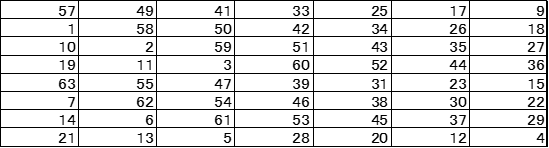
\includegraphics{syoki.png}
%     \caption{初期転置}
%     \label{figs}
%   \end{center}
% \end{figure}

分割された鍵をそれぞれ回転左シフトし、再結合する。\\
回転左シフトされた値\\
1110001010011101101100010110\\
1110001001000111110100101110\\
再結合された値
11100010100111011011000101101110001001000111110100101110

% ここにsyoki2.png

再結合された鍵を、{\tt test}を使用して転置を行う。また、これを拡大鍵とする。\\
拡大鍵
110110100000011010111111001001101101100001110010

\section{関数F}

分割された平文の右側と、拡大鍵を使用して関数Fの結果を求める。
初めに、分割された平文の右側を{\tt test}を使用して拡大転置を行う。
その後、転置された平文と拡大鍵の排他的論理和を求める。求めたビット列を{\tt test}のSBOXを参照して変換する。\\
平文右   11011 0001 0001 0001 0001 0001 0011 110


転置された平文
011011 110001 010001 010001 010001 010001 010011 111101\\
拡大鍵
110110 100000 011010 111111 001001 101101 100001 110010\\
排他的論理和をとった値
101101 010001 001011 101110 011000 111100 110010 001111\\
SBOXによって出た値\\
S1 1\\
S2 12\\
S3 4\\
S4 13\\
S5 13\\
S6 11\\
S7 15\\
S8 4


SBOXで求めた数値をそれぞれ二進数に変換する。\\
0001 1100 0100 1101 1101 1011 1111 0100


この値をさらに{\tt test}で転置を行った値が関数Fの値となる。\\
関数Fの値
10110011001111010011010001110011

\section{最終値}
最後に、関数Fで求めた数値と、分割された平文の左側の排他的論理和を求める。


平文左
01100000001000000010011001111010\\
関数F
10110011001111010011010001110011\\
最終値
11010011000111010001001000001001\\

% --- main content ---
\end{document}

